\documentclass{article}

\usepackage{graphicx}
\usepackage{float}
\usepackage{subcaption}

\title{My first document}
\date{2020-07-01}
\author{Christopher}

\begin{document}
	
	% orced picture to show where it is declared
	% options are:
	% h (here) - same location
	% H (Here) - same location but stricter (requires \usepackage{float})
    % t (top) - top of page
    % b (bottom) - bottom of page
    % p (page) - on an extra page
    % ! (override) - will force the specified location (doesn't support H)
	\begin{figure}[h!]
		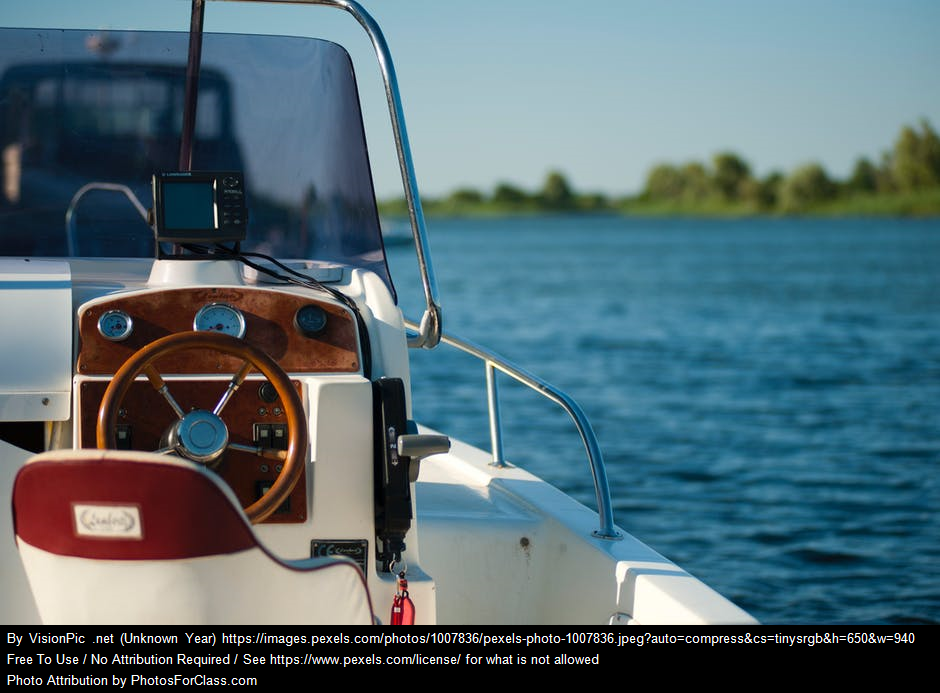
\includegraphics[width=\linewidth]{boat.png}
		\caption{A boat.}
		% invisible
		\label{fig:boat1}
	\end{figure}
	
	% might have to be compiled twice to work
	Figure \ref{fig:boat1} shows a boat.
	
	% multiple images
	\begin{figure}[h!]
		\centering
		%                    <- 40% of the page for each image (sum should always be less than 100%)
		\begin{subfigure}[b]{0.4\linewidth}
			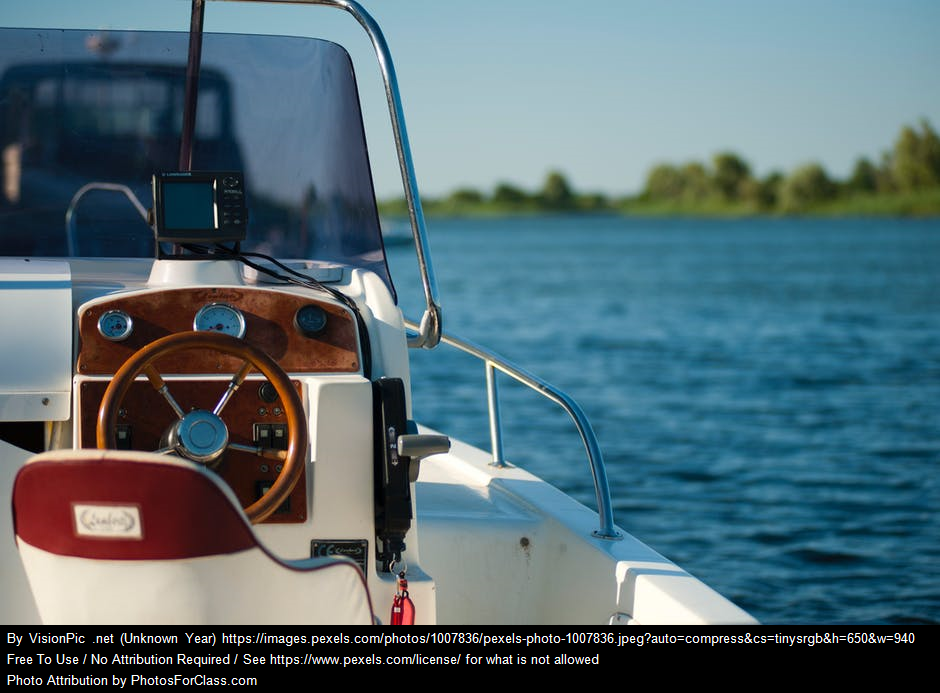
\includegraphics[width=\linewidth]{boat.png}
			\caption{Coffee.}
		\end{subfigure}
		\begin{subfigure}[b]{0.4\linewidth}
			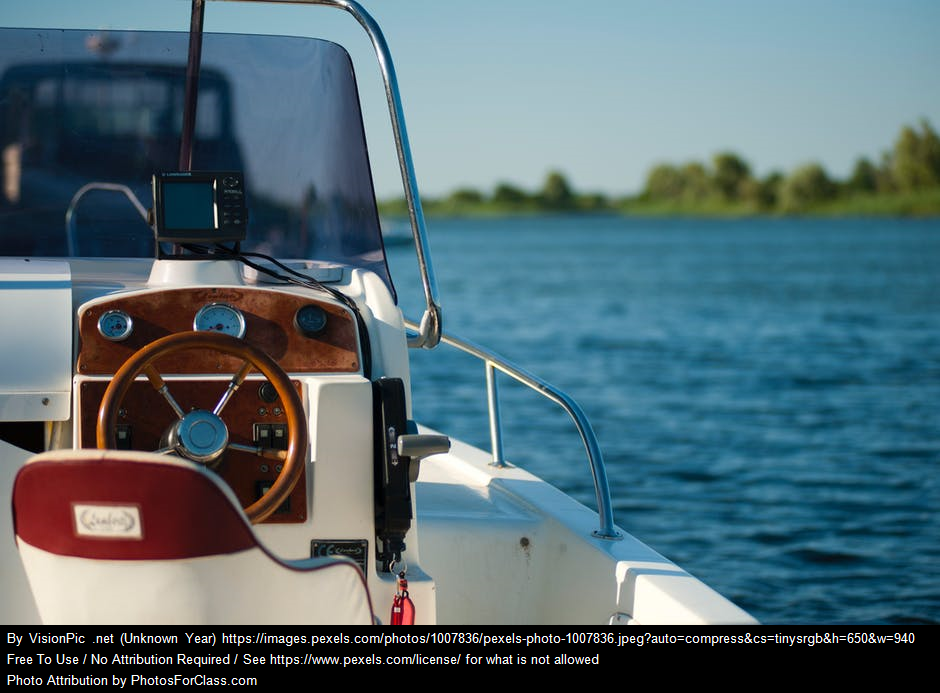
\includegraphics[width=\linewidth]{boat.png}
			\caption{More coffee.}
		\end{subfigure}
		\caption{The same cup of coffee. Two times.}
		\label{fig:coffee}
	\end{figure}
	
	% automated linebreak when the width is bigger than 100%	
	\begin{figure}[h!]
		\centering
		\begin{subfigure}[b]{0.2\linewidth}
			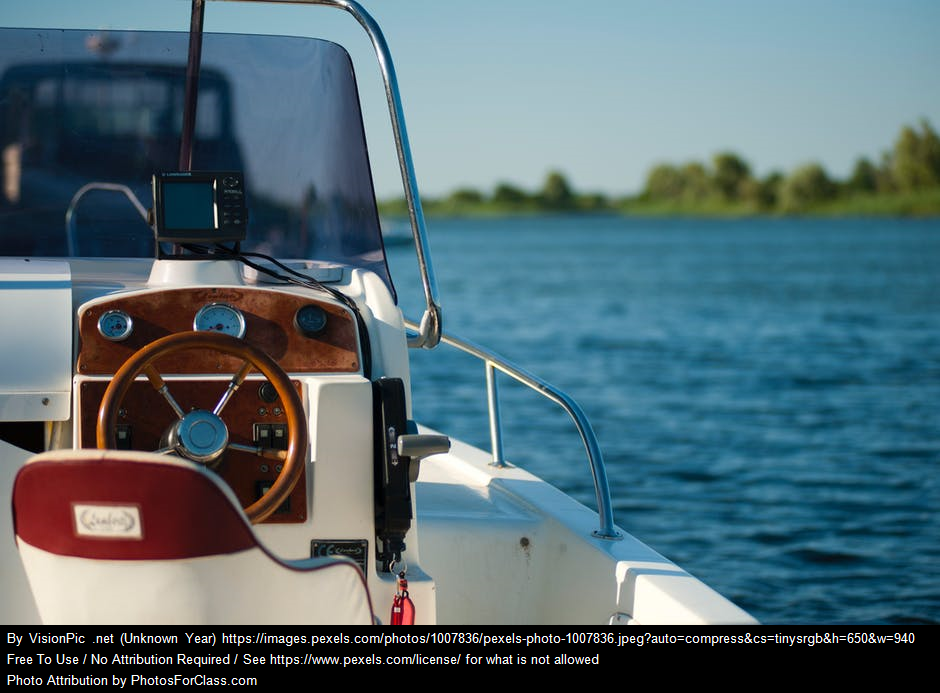
\includegraphics[width=\linewidth]{boat.png}
			\caption{Coffee.}
		\end{subfigure}
		\begin{subfigure}[b]{0.2\linewidth}
			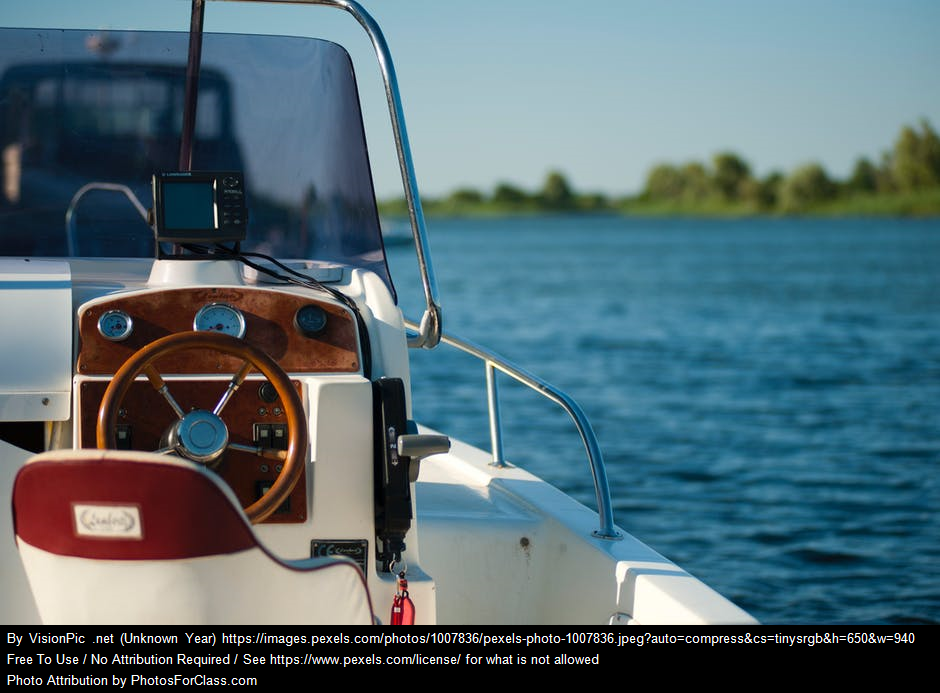
\includegraphics[width=\linewidth]{boat.png}
			\caption{More coffee.}
		\end{subfigure}
		\begin{subfigure}[b]{0.2\linewidth}
			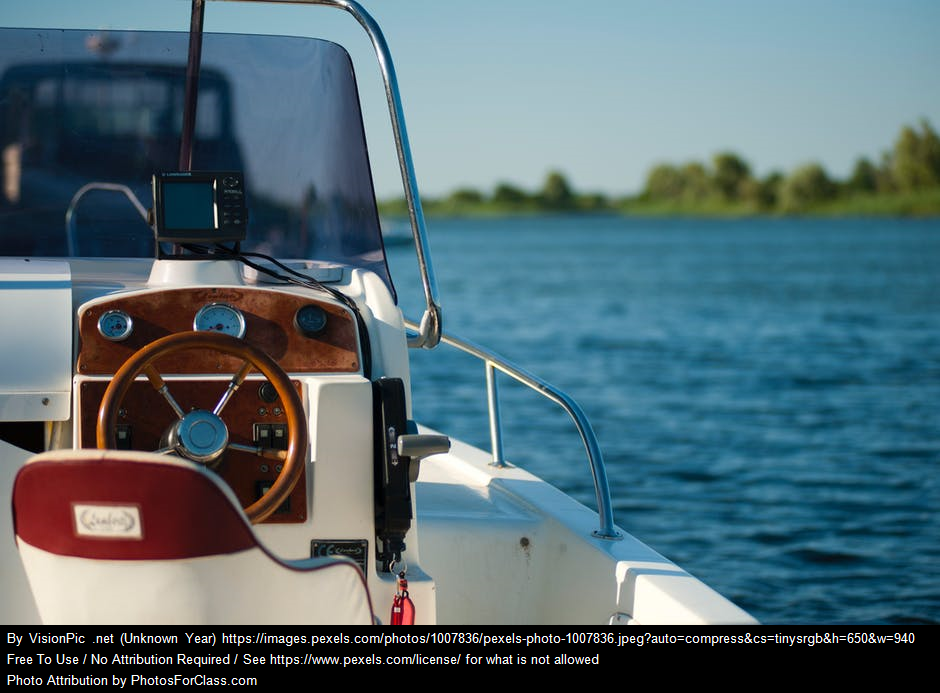
\includegraphics[width=\linewidth]{boat.png}
			\caption{Tasty coffee.}
		\end{subfigure}
		\begin{subfigure}[b]{0.5\linewidth}
			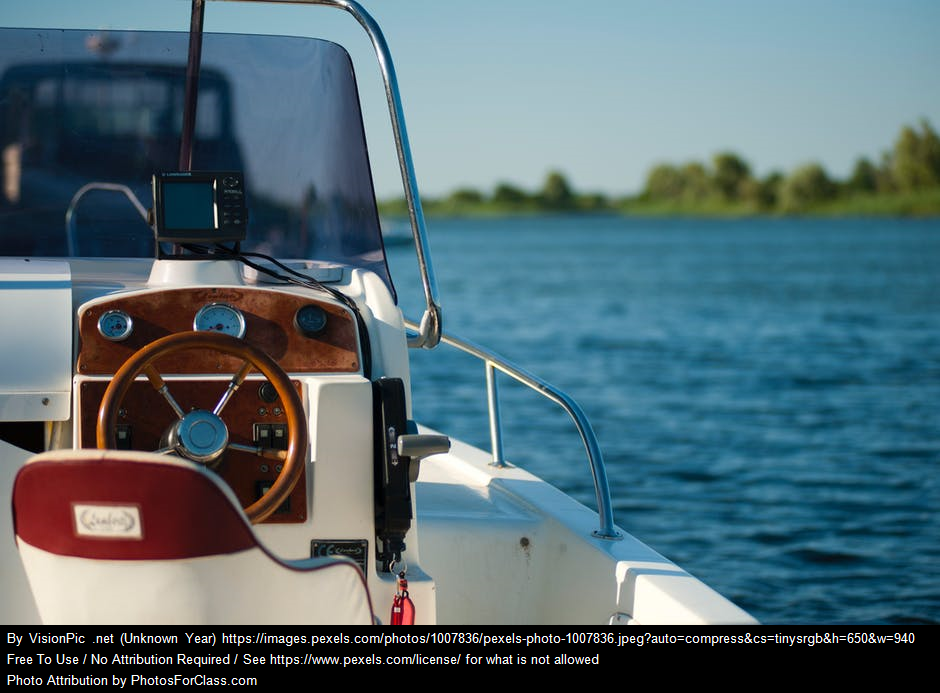
\includegraphics[width=\linewidth]{boat.png}
			\caption{Too much coffee.}
		\end{subfigure}
		\caption{The same cup of coffee. Multiple times.}
		\label{fig:coffee3}
	\end{figure}

\end{document}
